\chapter{Introdução ao Jamovi}

\section{O que é o Jamovi?}

O jamovi é um software estatístico com interface gráfica. É um software relativamente novo, se comparado com os seus concorrentes como o SPSS, SAS e PSPP. Com o jamovi você consegue ter um ambiente de fácil aprendizado e fácil manuseio, pois é possível integrar a facilidade do ambiente gráfico, com o poder da linguagem R para a automação de trabalhos.

Além das análises estatísticas convencionais, tais como: estatística descritiva, tabelas cruzadas, boxplot, etc. É possível desenvolver modelos matemáticos. Assim, podemos definir o jamovi como uma solução completa para análises quantitativas e qualitativas com o uso da matemática e estatística. Um software estatístico completo e gratuito.

\begin{figure}[H]
    \centering
    \caption{Captura de Tela do Jamovi}
    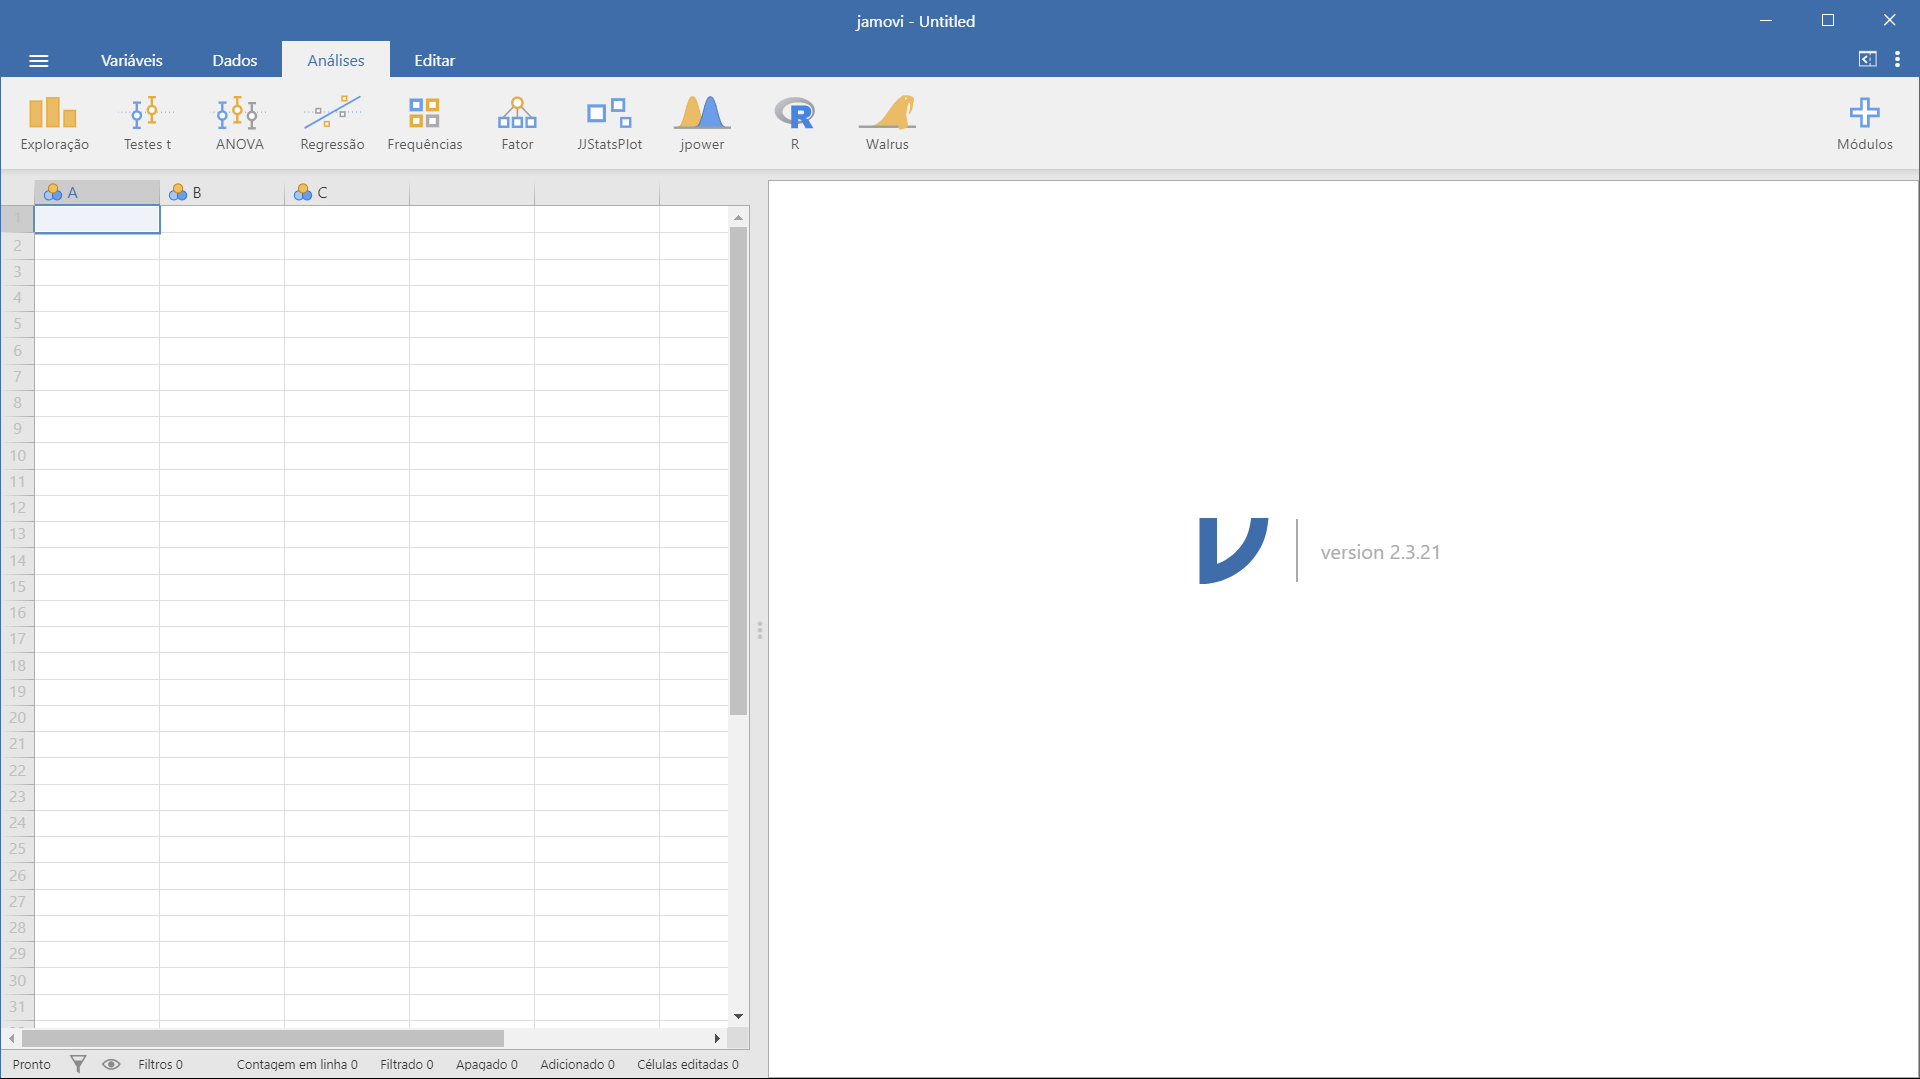
\includegraphics[width=\textwidth]{imagens/cap_1/captura_tela_jamovi.png}
    \label{fig:captura_tela_jamovi}
  \end{figure}

\subsection{Um software estatístico completo}

O jamovi é um dos softwares mais completos da atualidade. Sua interface gráfica e a integração com a linguagem de programação R, faz com que o programa seja capaz de realizar todas as análises, das mais simples até as mais importantes

Além de ser completo é um software open source e gratuito. Isso significa que você não precisa se preocupar em comprar licença e/ou fazer assinaturas. Além de ser gratuito, o fato de os códigos serem abertos, permite que todos e todas possam verificar diretamente no código fonte como o programa foi escrito, trazendo mais transparência e segurança para os(as) usuários(as)

\subsection{Estatística com interface gráfica}

Uma das principais barreiras para várias pessoas que desejam estudar estatística é a programação. Geralmente os(as) alunos(as) que estão começando a estudar estatística, estão começando também a ter o primeiro contato com a linguagem de programação

Uma das principais vantagens do Jamovi é sua interface gráfica. Com ela, o(a) aluno(a) que está começando nos estudos de estatística, pode se concentrar apenas no estudo teórico, deixando para outro momento o estudo da programação. Dessa forma, o jamovi é uma das melhores alternativas de software para estudos em estatística, pois permite que o(a) aluno(a) possa ver os resultados em tempo real, sem a necessidade de aprender os comandos de uma linguagem

\subsection{Software Modular}

O jamovi é um software modular. Isso significa que você pode instalar complementos, ou módulos de acordo com a sua necessidade. Diferentemente do SPSS, por exemplo, com o Jamovi você tem a liberdade de instalar somente os módulos que você precisa; algo que não é possível fazer no SPSS.

A liberdade de poder instalar os módulos, faz do Jamovi um software leve e personalizável. Além disso, a comunidade está ativamente desenvolvendo novos módulos, o que faz com que o Jamovi seja cada vez mais completo e flexível para atender diversos usuários

\subsection{Ambiente para aprender a linguagem R}

Apesar de ser um software com interface gráfica, o Jamovi tem integração com a linguagem de programação R. Isso significa que você tem a facilidade da interface gráfica, com o poder e a flexibilidade de uma das linguagens mais utilizadas no mundo da estatística.

Caso o Jamovi não tenha nativamente uma função que você precisa, você pode desenvolver utilizando a linguagem R. Essa integração faz com que seja possível realizar qualquer tipo de análise com o Jamovi. Além disso, você pode automatizar rotinas que são repetitivas e você precisa realizar várias vezes no seu trabalho e estudo.

\section{Instalação do Jamovi}

Para fazer a instalação do software Jamovi, é muito simples e dependerá apenas do sistema operacional em que você está utilizando.

Se você fizer a instalação no site oficial você não precisa se preocupar com a sua segurança e está livre para instalar e fazer o uso do programa da forma que você precisar. Não existe nenhum tipo de restrição quanto ao uso ou locais em que você deve instalar.

Assim, você é livre para fazer uso educacional, comercial ou qualquer outro motivo pois não há nenhum tipo de restrição quanto ao uso ou a licença do programa.

\subsection{Download do Jamovi}

Para você fazer a utilização do jamovi, existem duas possibilidades: uma em cloud sendo que você não precisa realizar nenhum tipo de instalação e pode utilizar o programa diretamente da internet; em uma opção localmente em que você pode fazer o download no seu computador e instalar como um programa qualquer.

As duas soluções são muito boas, entretanto eu aconselho que você faça a instalação no seu computador para que você tenha total controle sobre os dados e não corra o risco de perder dados na solução de nuvem.

Eu recomendo que você faça a utilização do programa em nuvem somente em casos em que você não tem a possibilidade de instalar o jamovi em seu computador.

Nas duas sessões posteriores vou ensinar para vocês um pouco de como prosseguir para fazer a utilização das duas formas.

\subsection{Jamovi para desktop}

Primeiramente é importante que você acesse a página oficial do Jamovi para fazer o download. Você pode acessá-la na seguinte página: \url{https://www.jamovi.org}. É fortemente aconselhável que você faça o download somente na página oficial. Vale lembrar que o Jamovi é gratuito e não é necessário recorrer e nenhum programa paralelo, ou site diferente do oficial.

Para fazer a instalação em seu computador você deve selecionar a opção correspondente para instalação no desktop. No momento em que eu preparo esse material o site está organizado da seguinte forma.

Ao entrar na parte de download você verá uma página como na figura \ref{fig:download_jamovi}.

\begin{figure}[H]
  \centering
  \caption{Opção de Download do Jamovi para Desktop}
  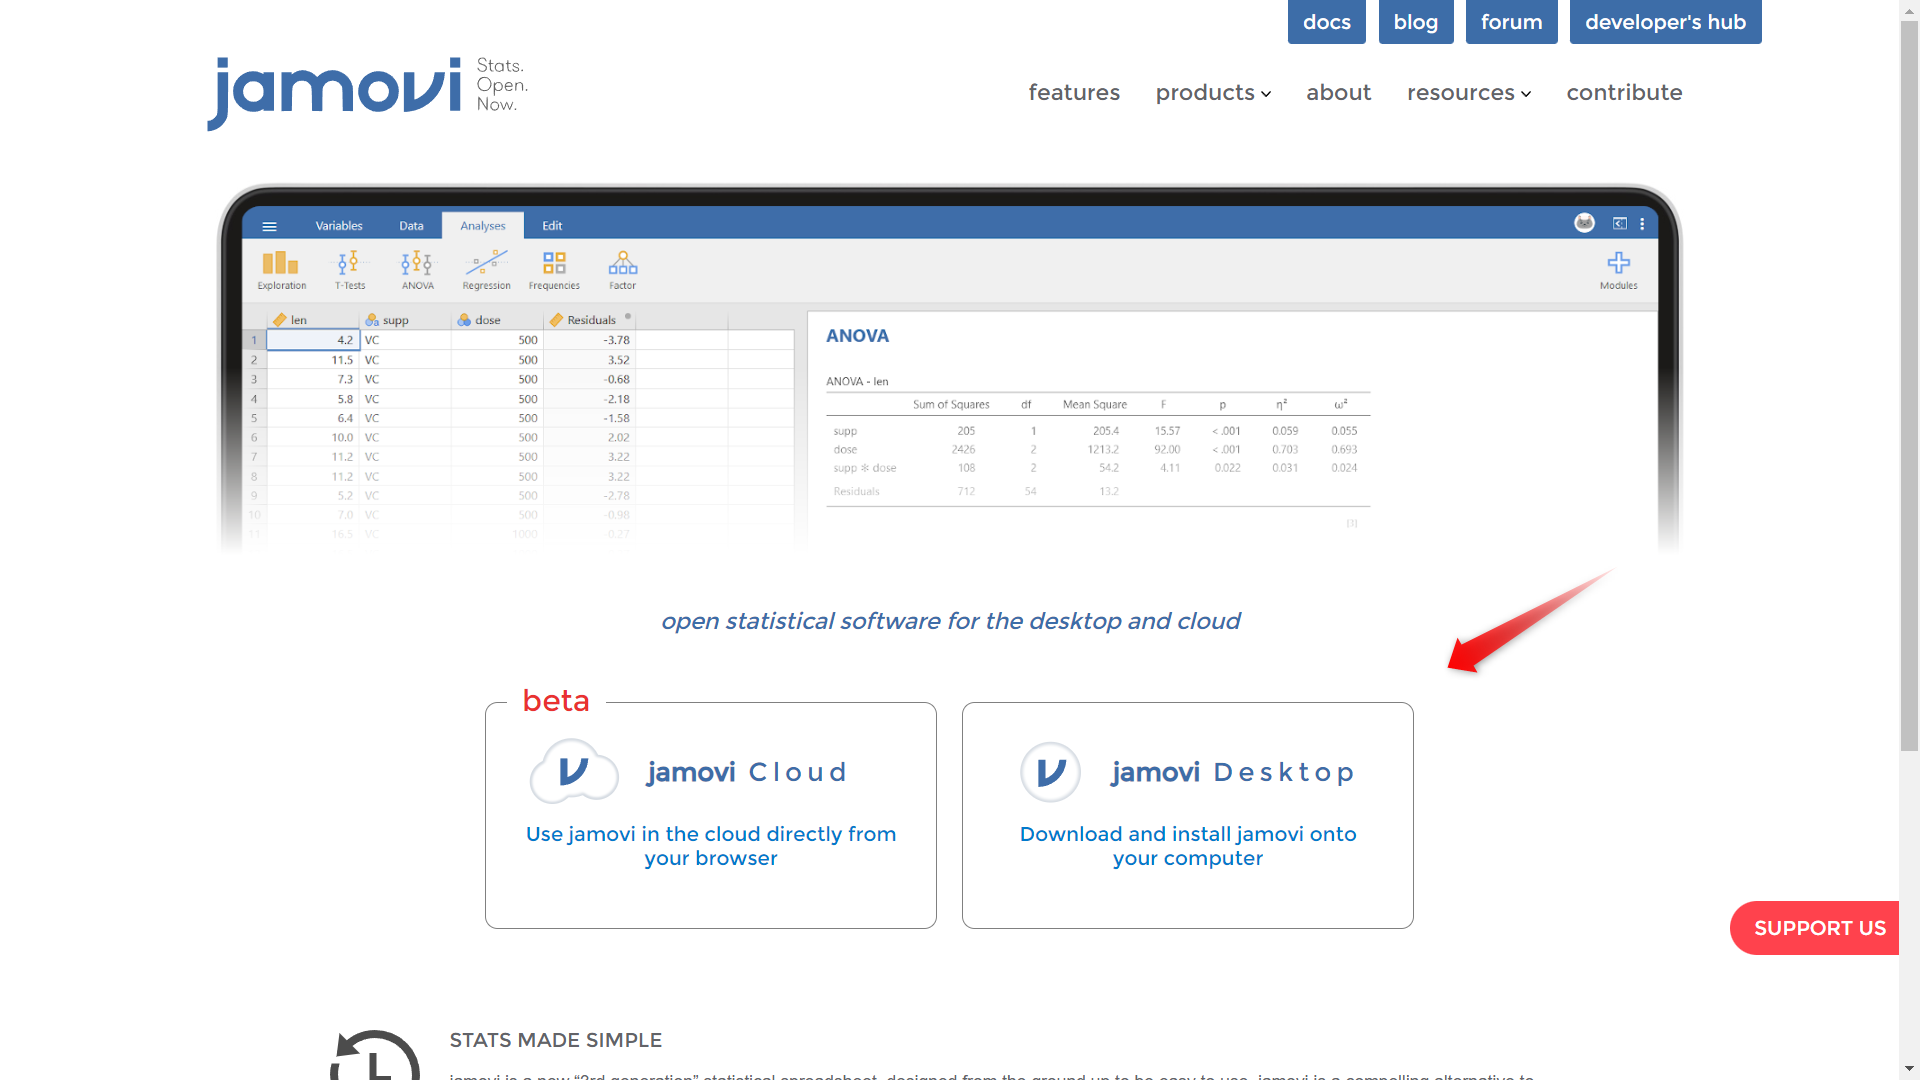
\includegraphics[width=\textwidth]{imagens/cap_1/download_jamovi.png}
  \label{fig:download_jamovi}
\end{figure}

Selecione a opção desktop conforme indicado na imagem \ref{fig:download_jamovi} com uma seta. Ao clicar avance para o próximo tópico da apostila, pois vamos selecionar a versão do Jamovi que será instalada.

\subsection{Selecionando a versão do Jamovi}

Para fazer o download do Jamovi em seu computador, você precisa selecionar a versão correspondente ao seu sistema operacional. É importante que você faça a escolha correta, pois caso você cometa um equívoco na escola o programa não funcionará, ou não funcionará corretamente.

Geralmente quando você chegar na página de download, o próprio site já irá indicar a versão correta, correspondente ao seu sistema operacional. Basta você conferir e prosseguir para o download do programa.

Caso a sugestão do site esteja errada, basta rolar a página um pouco para baixo e selecionar a versão correta correspondente, assim como mostrado na imagem abaixo.

\begin{figure}[H]
  \centering
  \caption{Seleciona a versão do Jamovi}
  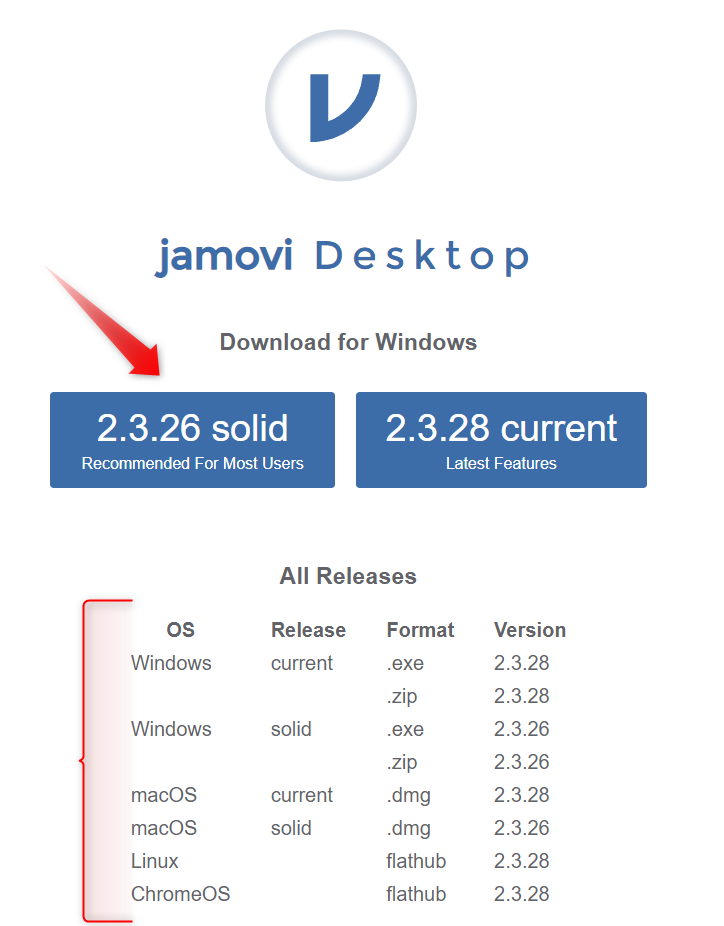
\includegraphics[width=0.5\textwidth]{imagens/cap_1/seleciona_versao_jamovi.png}
  \label{fig:download_jamovi}
\end{figure}

